% ============================================================
%  Příprava na maturitu – Elektrotechnika
%  Okruh 1: Stejnosměrný proud, základy elektrochemie
% ============================================================

\documentclass[a4paper,10pt]{article}

\usepackage[T1]{fontenc}
\usepackage[utf8]{inputenc}
\usepackage[left=2.0cm, right=1.8cm, top=1.8cm, bottom=1.8cm]{geometry}
\usepackage{parskip}
\usepackage{xcolor}
\usepackage{tabularx}
\usepackage{booktabs}
\usepackage{tikz}
\usepackage{mdframed}
\usepackage{amsmath}
\usepackage{enumitem}
\usepackage{circuitikz}

\usetikzlibrary{arrows.meta, positioning, decorations.pathmorphing, shapes.geometric}

% --- Barvy ---
\definecolor{accent}{HTML}{1A3A5C}
\definecolor{lightblue}{HTML}{EAF2F8}
\definecolor{lightyellow}{HTML}{FDFBE4}
\definecolor{lightgreen}{HTML}{EAF7EA}
\definecolor{lightred}{HTML}{FDE8E8}
\definecolor{lightgray}{HTML}{F4F4F4}

% --- Boxy ---
\newmdenv[backgroundcolor=lightblue,linecolor=accent!40,roundcorner=4pt,
  innertopmargin=6pt,innerbottommargin=6pt,innerleftmargin=8pt,innerrightmargin=8pt]{pojmybox}
\newmdenv[backgroundcolor=lightyellow,linecolor=accent!30,roundcorner=4pt,
  innertopmargin=6pt,innerbottommargin=6pt,innerleftmargin=8pt,innerrightmargin=8pt]{vysvetlenibox}
\newmdenv[backgroundcolor=lightgreen,linecolor=accent!40,roundcorner=4pt,
  innertopmargin=6pt,innerbottommargin=6pt,innerleftmargin=8pt,innerrightmargin=8pt]{vzorcebox}
\newmdenv[backgroundcolor=lightred,linecolor=accent!30,roundcorner=4pt,
  innertopmargin=6pt,innerbottommargin=6pt,innerleftmargin=8pt,innerrightmargin=8pt]{durazbox}

\setlist[itemize]{noitemsep, leftmargin=1.4em, topsep=2pt}
\setlist[enumerate]{noitemsep, leftmargin=1.4em, topsep=2pt}

% --- Zkratka pro jednotky ---
\newcommand{\jednotka}[1]{\,[\mathrm{#1}]}

\begin{document}

% ============================================================
\section*{\large Okruh 1 – Stejnosměrný proud, základy elektrochemie}

\begin{pojmybox}
\textbf{Klíčové pojmy:}
elektrický náboj, elektrický proud, napětí, odpor, Ohmův zákon, výkon, práce, Kirchhoffovy zákony,
sériové/paralelní zapojení, elektrický článek, akumulátor, elektrolýza, Faradayovy zákony, galvanické pokovování
\end{pojmybox}

\begin{vysvetlenibox}

% ================================================================
\subsection*{1. Elektrický náboj a proud}

\textbf{Elektrický náboj} $Q$ je základní vlastnost hmoty; nositeli jsou elektrony (záporné) a protony (kladné).

\begin{vzorcebox}
\[
Q = I \cdot t \jednotka{C}
\quad\quad
I = \frac{Q}{t} \jednotka{A}
\]
kde $Q$ = náboj [C = A$\cdot$s], $I$ = proud [A], $t$ = čas [s].
\end{vzorcebox}

\textbf{Stejnosměrný proud (DC)} – elektrony se pohybují stále jedním směrem (od $-$ k $+$ pólu zdroje).

\medskip
\begin{center}
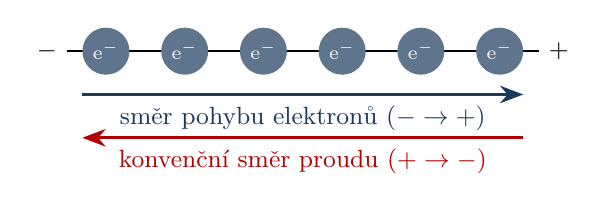
\begin{tikzpicture}[>=Stealth, font=\small]
  % Vodiče
  \draw[thick] (0,0) -- (6,0);
  % Elektrony jedoucí zleva doprava
  \foreach \x in {0.5, 1.5, 2.5, 3.5, 4.5, 5.5} {
    \node[circle, fill=accent!70, text=white, inner sep=2pt] at (\x, 0) {\scriptsize e$^-$};
  }
  \draw[->, thick, accent, line width=1.2pt] (0.2,-0.55) -- (5.8,-0.55)
    node[midway, below, text=accent] {směr pohybu elektronů ($-\to+$)};
  \draw[->, thick, red!70!black, line width=1.2pt] (5.8,-1.1) -- (0.2,-1.1)
    node[midway, below, text=red!70!black] {konvenční směr proudu ($+\to-$)};
  % Popis
  \node[left] at (0,0) {\textbf{$-$}};
  \node[right] at (6,0) {\textbf{$+$}};
\end{tikzpicture}
\end{center}

% ================================================================
\subsection*{2. Elektrické napětí a odpor}

\textbf{Elektrické napětí} $U$ je práce vykonaná na přenesení jednotkového náboje mezi dvěma body.
\textbf{Elektrický odpor} $R$ vyjadřuje, jak moc materiál brání průchodu proudu.

\begin{vzorcebox}
\[
U = \frac{W}{Q} \jednotka{V}
\qquad
R = \rho \cdot \frac{l}{S} \jednotka{\Omega}
\]
kde $W$ = práce [J], $\rho$ = měrný odpor [$\Omega\cdot$m], $l$ = délka vodiče [m], $S$ = průřez vodiče [m$^2$].
\end{vzorcebox}

% ================================================================
\subsection*{3. Ohmův zákon}

\begin{vzorcebox}
\[
U = R \cdot I
\qquad
I = \frac{U}{R}
\qquad
R = \frac{U}{I}
\]
\end{vzorcebox}

Platí pro lineární (ohmické) součástky při konstantní teplotě.

\medskip
\begin{center}
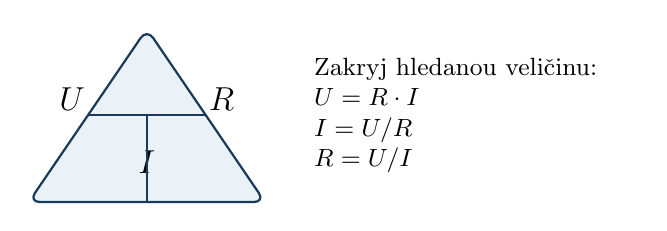
\begin{tikzpicture}[font=\small, >=Stealth]
  % Ohmův trojúhelník
  \draw[thick, accent, fill=lightblue, rounded corners=4pt]
    (0,0) -- (3,0) -- (1.5,2.2) -- cycle;
  \node[font=\large\bfseries] at (1.5,0.5) {$I$};
  \node[font=\large\bfseries] at (0.55,1.3) {$U$};
  \node[font=\large\bfseries] at (2.45,1.3) {$R$};
  % Dělicí čára
  \draw[thick, accent] (0.75,1.1) -- (2.25,1.1);
  \draw[thick, accent] (1.5,0) -- (1.5,1.1);
  % Popis
  \node[right, text width=4cm] at (3.5,1.1)
    {Zakryj hledanou veličinu:\\ $U = R \cdot I$\\ $I = U / R$\\ $R = U / I$};
\end{tikzpicture}
\end{center}

% ================================================================
\subsection*{4. Výkon a elektrická práce}

\begin{vzorcebox}
\[
P = U \cdot I = \frac{U^2}{R} = I^2 \cdot R \jednotka{W}
\qquad
W = P \cdot t = U \cdot I \cdot t \jednotka{J}
\]
\end{vzorcebox}

Praktická jednotka práce: $1\,\mathrm{kWh} = 3{,}6 \cdot 10^6\,\mathrm{J}$.

% ================================================================
\subsection*{5. Zapojení odporů}

\subsubsection*{Sériové zapojení}

\begin{center}
\begin{circuitikz}[font=\small]
  \draw (0,0)
    to[short, o-] (0.5,0)
    to[R, l=$R_1$] (2.5,0)
    to[R, l=$R_2$] (4.5,0)
    to[R, l=$R_3$] (6.5,0)
    to[short, -o] (7,0);
  \node[below] at (0,0) {$U$};
  \draw[->, thick, red!70!black] (0.2,-0.6) -- (6.8,-0.6)
    node[midway, below] {$I$ – stejný všude};
\end{circuitikz}
\end{center}

\begin{vzorcebox}
\[
R_{celk} = R_1 + R_2 + R_3 + \cdots
\qquad
U_{celk} = U_1 + U_2 + U_3
\qquad
I = \text{const.}
\]
\end{vzorcebox}

\subsubsection*{Paralelní zapojení}

\begin{center}
\begin{circuitikz}[font=\small]
  \draw (0,1.5)
    to[short, o-] (1,1.5)
    to[short] (1,3)
    to[R, l=$R_1$] (4,3)
    to[short] (4,1.5);
  \draw (1,1.5)
    to[R, l=$R_2$] (4,1.5);
  \draw (1,1.5)
    to[short] (1,0)
    to[R, l=$R_3$] (4,0)
    to[short] (4,1.5)
    to[short, -o] (5,1.5);
  \node[left] at (0,1.5) {$U$};
  \node[below] at (2.5,-0.5) {$U$ – stejné na všech větvích};
\end{circuitikz}
\end{center}

\begin{vzorcebox}
\[
\frac{1}{R_{celk}} = \frac{1}{R_1} + \frac{1}{R_2} + \frac{1}{R_3}
\qquad
\text{(pro 2 odpory: } R_{celk} = \frac{R_1 \cdot R_2}{R_1 + R_2} \text{)}
\]
\[
I_{celk} = I_1 + I_2 + I_3
\qquad
U = \text{const.}
\]
\end{vzorcebox}

\begin{center}
\begin{tabularx}{0.85\linewidth}{@{} l X X @{}}
\toprule
\textbf{Vlastnost} & \textbf{Sériové} & \textbf{Paralelní} \\
\midrule
Proud & stejný ve všech prvcích & dělí se do větví \\
Napětí & dělí se na prvcích & stejné na všech větvích \\
Celkový odpor & větší než největší $R$ & menší než nejmenší $R$ \\
Výpadek prvku & přeruší celý obvod & ostatní větve fungují dál \\
\bottomrule
\end{tabularx}
\end{center}

% ================================================================
\subsection*{6. Kirchhoffovy zákony}

\begin{durazbox}
\textbf{1. Kirchhoffův zákon (KCL) – o uzlech:}\\
Součet proudů vstupujících do uzlu se rovná součtu proudů vystupujících z uzlu.
\[
\sum I_{vst} = \sum I_{vyst}
\qquad \Leftrightarrow \qquad \sum I = 0
\]

\medskip
\textbf{2. Kirchhoffův zákon (KVL) – o smyčkách:}\\
Součet všech napětí ve smyčce je roven nule (součet napětí zdrojů = součet úbytků napětí).
\[
\sum U = 0
\qquad \Leftrightarrow \qquad \sum U_{zdroj} = \sum U_{ubytek}
\]
\end{durazbox}

\begin{center}
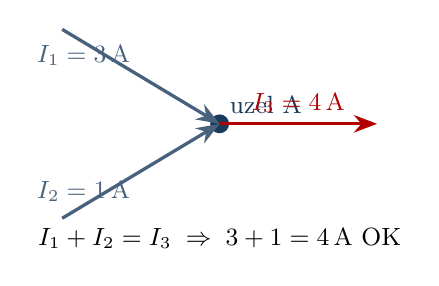
\begin{tikzpicture}[font=\small, >=Stealth, thick]
  % Uzel
  \filldraw[accent] (2,2) circle (3pt) node[above right] {uzel A};
  % Proudy
  \draw[->, accent!80, line width=1.2pt] (0,3.2) -- (2,2)
    node[midway, above left] {$I_1 = 3\,\mathrm{A}$};
  \draw[->, accent!80, line width=1.2pt] (0,0.8) -- (2,2)
    node[midway, below left] {$I_2 = 1\,\mathrm{A}$};
  \draw[->, red!70!black, line width=1.2pt] (2,2) -- (4,2)
    node[midway, above] {$I_3 = 4\,\mathrm{A}$};
  \node[below] at (2,0.8) {$I_1 + I_2 = I_3 \;\Rightarrow\; 3+1=4\,\mathrm{A}$ OK};
\end{tikzpicture}
\end{center}

% ================================================================
\subsection*{7. Zdroje stejnosměrného napětí – elektrické články}

\textbf{Galvanický článek} přeměňuje chemickou energii na elektrickou pomocí redox reakcí na elektrodách ponořených v elektrolytu.

\begin{center}
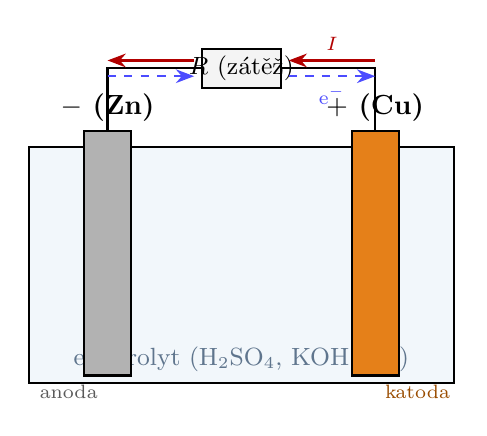
\begin{tikzpicture}[font=\small, >=Stealth]
  % Nádoba s elektrolytem
  \draw[thick, fill=lightblue!60] (0.3,0) rectangle (5.7,3);
  \node[text=accent!70] at (3,0.3) {elektrolyt (H$_2$SO$_4$, KOH, \ldots)};

  % Záporná elektroda (anoda – Zn)
  \draw[thick, fill=gray!60] (1,0.1) rectangle (1.6,3.2);
  \node[above, font=\bfseries] at (1.3,3.2) {$-$ (Zn)};
  \node[below left, text=gray!70!black, font=\scriptsize] at (1.3,0.1)
    {anoda};

  % Kladná elektroda (katoda – Cu)
  \draw[thick, fill=orange!60!brown] (4.4,0.1) rectangle (5,3.2);
  \node[above, font=\bfseries] at (4.7,3.2) {$+$ (Cu)};
  \node[below right, text=orange!60!black, font=\scriptsize] at (4.7,0.1)
    {katoda};

  % Spojovací vodič + odpor (zátěž)
  \draw[thick] (1.3,3.2) -- (1.3,4) -- (4.7,4) -- (4.7,3.2);
  \draw[thick, fill=lightgray] (2.5,3.75) rectangle (3.5,4.25);
  \node at (3,4) {$R$ (zátěž)};

  % Šipka proudu
  \draw[->, red!70!black, thick] (4.7,4.1) -- (3.6,4.1)
    node[above, midway, font=\scriptsize] {$I$};
  \draw[->, red!70!black, thick] (2.4,4.1) -- (1.3,4.1);

  % Elektrony opačně
  \draw[->, blue!70, thick, dashed] (1.3,3.9) -- (2.4,3.9);
  \draw[->, blue!70, thick, dashed] (3.6,3.9) -- (4.7,3.9)
    node[below, midway, font=\scriptsize, text=blue!70] {e$^-$};
\end{tikzpicture}
\end{center}

\textbf{Parametry zdroje:}
\begin{itemize}
  \item \textbf{EMF} (elektromotorická síla) $\varepsilon$ – napětí naprázdno [V]
  \item \textbf{Vnitřní odpor} $R_i$ – způsobuje úbytek napětí při zatížení
  \item \textbf{Svorkové napětí:} $U = \varepsilon - R_i \cdot I$
\end{itemize}

\begin{vzorcebox}
\[
U_{svorky} = \varepsilon - R_i \cdot I
\]
\end{vzorcebox}

% ================================================================
\subsection*{8. Typy elektrochemických zdrojů}

\begin{center}
\begin{tabularx}{0.97\linewidth}{@{} l X X X @{}}
\toprule
\textbf{Typ} & \textbf{Princip} & \textbf{Nabíjitelný?} & \textbf{Příklady} \\
\midrule
Primární článek & jednorázová reakce & Ne & tužková baterie (Zn-MnO$_2$) \\
Sekundární článek (akumulátor) & reversibilní reakce & Ano & Li-ion, NiMH, olověný \\
Palivový článek & přísun paliva (H$_2$) & kontinuální & elektromobily, záložní zdroje \\
\bottomrule
\end{tabularx}
\end{center}

\subsubsection*{Olověný akumulátor}

Nejrozšířenější akumulátor (autobaterie). Elektrody: Pb (záporná) a PbO$_2$ (kladná), elektrolyt: H$_2$SO$_4$ (kyselina sírová).

\begin{center}
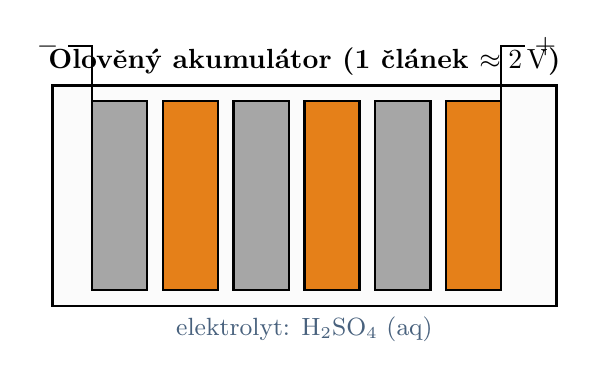
\begin{tikzpicture}[font=\small, >=Stealth]
  % Skříň
  \draw[thick, fill=lightgray!40] (-0.2,-0.3) rectangle (6.2,2.5);
  \node[above, font=\bfseries] at (3,2.5) {Olověný akumulátor (1 článek $\approx 2\,\mathrm{V}$)};

  % Elektrody (střídavě Pb a PbO2)
  \foreach \x/\col/\lbl in {0.3/gray!70/{Pb ($-$)}, 1.2/orange!60!brown/{PbO$_2$ ($+$)},
                              2.1/gray!70/{Pb ($-$)}, 3.0/orange!60!brown/{PbO$_2$ ($+$)},
                              3.9/gray!70/{Pb ($-$)}, 4.8/orange!60!brown/{PbO$_2$ ($+$)}} {
    \draw[thick, fill=\col] (\x,-0.1) rectangle (\x+0.7,2.3);
  }

  % Elektrolyt popis
  \node[text=accent!80] at (3,-0.6) {elektrolyt: H$_2$SO$_4$ (aq)};

  % Svorkové kontakty
  \draw[thick] (0.3,2.3) -- (0.3,3) -- (0,3);
  \node[left, font=\bfseries] at (0,3) {$-$};
  \draw[thick] (5.5,2.3) -- (5.5,3) -- (5.8,3);
  \node[right, font=\bfseries] at (5.8,3) {$+$};
\end{tikzpicture}
\end{center}

\textbf{Reakce při vybíjení:}
\[
\text{Pb} + \text{PbO}_2 + 2\,\text{H}_2\text{SO}_4 \;\longrightarrow\; 2\,\text{PbSO}_4 + 2\,\text{H}_2\text{O}
\]
Při nabíjení reakce probíhá opačně (dodáme elektrickou energii).

% ================================================================
\subsection*{9. Elektrolýza}

Elektrolýza je rozklad chemické sloučeniny průchodem elektrického proudu.

\begin{center}
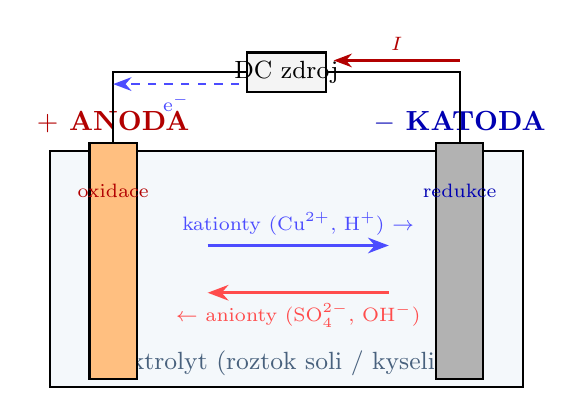
\begin{tikzpicture}[font=\small, >=Stealth, thick]
  % Nádoba
  \draw[fill=lightblue!50] (0.5,0) rectangle (6.5,3);
  \node[text=accent!80] at (3.5,0.3) {elektrolyt (roztok soli / kyseliny)};

  % Anoda (+)
  \draw[fill=orange!50] (1,0.1) rectangle (1.6,3.1);
  \node[above, font=\bfseries, text=red!70!black] at (1.3,3.1) {$+$ ANODA};
  \node[font=\scriptsize, text=red!70!black] at (1.3,2.5) {oxidace};

  % Katoda (-)
  \draw[fill=gray!60] (5.4,0.1) rectangle (6,3.1);
  \node[above, font=\bfseries, text=blue!70!black] at (5.7,3.1) {$-$ KATODA};
  \node[font=\scriptsize, text=blue!70!black] at (5.7,2.5) {redukce};

  % Kationty → katoda
  \draw[->, blue!70, line width=1pt] (2.5,1.8) -- (4.8,1.8)
    node[midway, above, font=\scriptsize] {kationty (Cu$^{2+}$, H$^+$) $\to$};

  % Anionty → anoda
  \draw[->, red!70, line width=1pt] (4.8,1.2) -- (2.5,1.2)
    node[midway, below, font=\scriptsize] {$\leftarrow$ anionty (SO$_4^{2-}$, OH$^-$)};

  % Zdroj napájení
  \draw (1.3,3.1) -- (1.3,4) -- (3.5,4);
  \draw (5.7,3.1) -- (5.7,4) -- (3.5,4);
  \draw[fill=lightgray] (3,3.75) rectangle (4,4.25);
  \node at (3.5,4) {DC zdroj};
  \draw[->, red!70!black] (5.7,4.15) -- (4.1,4.15)
    node[above, midway, font=\scriptsize] {$I$};
  \draw[->, blue!70, dashed] (2.9,3.85) -- (1.3,3.85)
    node[below, midway, font=\scriptsize, text=blue!70] {e$^-$};
\end{tikzpicture}
\end{center}

\begin{itemize}
  \item \textbf{Katoda} ($-$) – přitahuje kationty, probíhá \textbf{redukce} (přijímání elektronů)\\
    příklad: Cu$^{2+}$ + 2e$^-$ → Cu (usazení mědi)
  \item \textbf{Anoda} ($+$) – přitahuje anionty, probíhá \textbf{oxidace} (odevzdávání elektronů)\\
    příklad: Cu → Cu$^{2+}$ + 2e$^-$ (rozpouštění anody)
\end{itemize}

% ================================================================
\subsection*{10. Faradayovy zákony elektrolýzy}

\begin{vzorcebox}
\textbf{1. Faradayův zákon:} Hmotnost vyloučené látky je přímo úměrná prošlému náboji.
\[
m = A \cdot Q = A \cdot I \cdot t
\]

\textbf{2. Faradayův zákon:} Hmotnosti vyloučených látek stejným nábojem jsou úměrné jejich ekvivalentním hmotnostem.
\[
m = \frac{M \cdot I \cdot t}{z \cdot F}
\]
kde:
\begin{itemize}
  \item $m$ = hmotnost vyloučené látky [g]
  \item $M$ = molární hmotnost [g/mol]
  \item $I$ = proud [A], $t$ = čas [s]
  \item $z$ = mocenství iontu (počet vyměněných elektronů)
  \item $F = 96\,485\,\mathrm{C/mol}$ = Faradayova konstanta
\end{itemize}
\end{vzorcebox}

\textbf{Příklad:} Kolik mědi se vyloučí za 1 hodinu při proudu 2 A?
($M_{Cu} = 63{,}5\,\mathrm{g/mol}$, $z = 2$)
\[
m = \frac{63{,}5 \cdot 2 \cdot 3600}{2 \cdot 96485} \approx 2{,}37\,\mathrm{g}
\]

% ================================================================
\subsection*{11. Využití elektrolýzy – galvanické pokovování}

Galvanické pokovování nanáší tenkou vrstvu kovu (Cr, Ni, Au, Cu, Zn) na základní materiál pro ochranu nebo estetiku.

\begin{center}
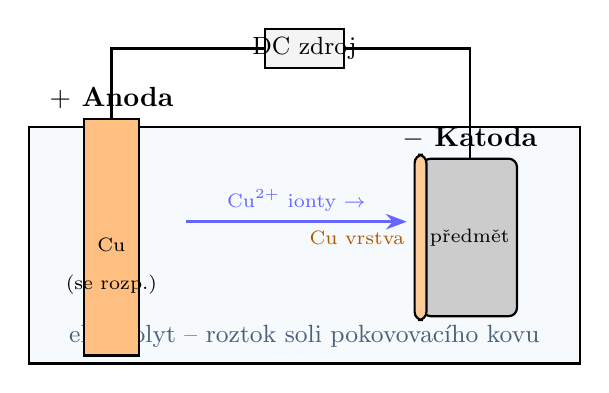
\begin{tikzpicture}[font=\small, >=Stealth, thick]
  % Vana
  \draw[fill=lightblue!40] (0,0) rectangle (7,3);
  \node[text=accent!80] at (3.5,0.35) {elektrolyt – roztok soli pokovovacího kovu};

  % Anoda – pokovovací kov
  \draw[fill=orange!50] (0.7,0.1) rectangle (1.4,3.1);
  \node[above, font=\bfseries] at (1.05,3.1) {$+$ Anoda};
  \node[font=\scriptsize] at (1.05,1.5) {Cu};
  \node[font=\scriptsize] at (1.05,1.0) {(se rozp.)};

  % Katoda – pokovovaný předmět
  \draw[thick, fill=gray!40, rounded corners=3pt] (5,0.6) rectangle (6.2,2.6);
  \node[above, font=\bfseries] at (5.6,2.6) {$-$ Katoda};
  \node[font=\scriptsize] at (5.6,1.6) {předmět};

  % Vrstva Cu na katodě
  \draw[thick, fill=orange!40, rounded corners=3pt] (4.9,0.55) rectangle (5.05,2.65);
  \node[left, font=\scriptsize, text=orange!70!black] at (4.9,1.6) {Cu vrstva};

  % Ionty Cu2+
  \draw[->, blue!60, line width=1pt] (2,1.8) -- (4.8,1.8)
    node[midway, above, font=\scriptsize] {Cu$^{2+}$ ionty $\to$};

  % Zdroj
  \draw (1.05,3.1) -- (1.05,4) -- (3.5,4);
  \draw (5.6,2.6) -- (5.6,4) -- (3.5,4);
  \draw[fill=lightgray] (3,3.75) rectangle (4,4.25);
  \node at (3.5,4) {DC zdroj};
\end{tikzpicture}
\end{center}

\textbf{Využití:}
\begin{itemize}
  \item ochrana před korozí (pozinkování, pochromování)
  \item dekorativní účely (zlatení, stříbření)
  \item výroba plošných spojů (měděné spoje)
  \item opravy a renovace kovových dílů
\end{itemize}

% ================================================================
\subsection*{12. Shrnutí – přehled vzorců}

\begin{center}
\begin{tabularx}{0.97\linewidth}{@{} l l l @{}}
\toprule
\textbf{Veličina} & \textbf{Vzorec} & \textbf{Jednotka} \\
\midrule
Náboj & $Q = I \cdot t$ & C (coulomb) \\
Napětí & $U = R \cdot I$ & V (volt) \\
Odpor (Ohm) & $R = U / I$ & $\Omega$ (ohm) \\
Odpor (mat.) & $R = \rho \cdot l / S$ & $\Omega$ \\
Výkon & $P = U \cdot I = I^2 R = U^2/R$ & W (watt) \\
Práce & $W = P \cdot t$ & J (joule) \\
Svorkové napětí & $U = \varepsilon - R_i \cdot I$ & V \\
Faraday & $m = \dfrac{M \cdot I \cdot t}{z \cdot F}$ & g \\
Sériový $R$ & $R_{celk} = R_1 + R_2 + \cdots$ & $\Omega$ \\
Paralelní $R$ & $1/R_{celk} = 1/R_1 + 1/R_2 + \cdots$ & $\Omega$ \\
\bottomrule
\end{tabularx}
\end{center}

\end{vysvetlenibox}

\end{document}
